\section{W8-10: Transport Layer}

\subsection{Transmission Control Protocol (TCP)}
\textbf{Connection-oriented:} three-way handshake.\\
\textbf{Congestion control:} slow start, congestion avoidance, fast retransmit, fast recovery.\\
\textbf{Full duplex:} two-way simultaneous data transfer.\\
\textbf{Sliding window protocol:} sender maintains a window of sent but unacknowledged packets. Reliable data delivery without overloading the receiver.\\
\textbf{TCP headers:} source port, destination port, sequence number (if SYN = 1, initial sequence number. If SYN = 0, sequence number of first data byte in this segment), acknowledgement number (if ACK = 1, next sequence number that the sender of the ACK is expecting), data offset (size of TCP header $20 \text{ bytes} = 5 \times 32 \text{-bits}$ to $60 \text{ bytes} = 15 \times 32 \text{-bits}$), flags (single bit flags), window size (how much data the sender of this segment is willing to receive).\\
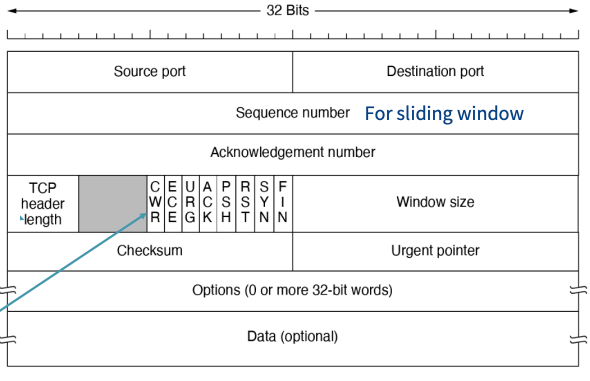
\includegraphics[width=\linewidth]{figs/tcp-header.png}
\textbf{Three-way handshake:} SYN, SYN-ACK, ACK.\\
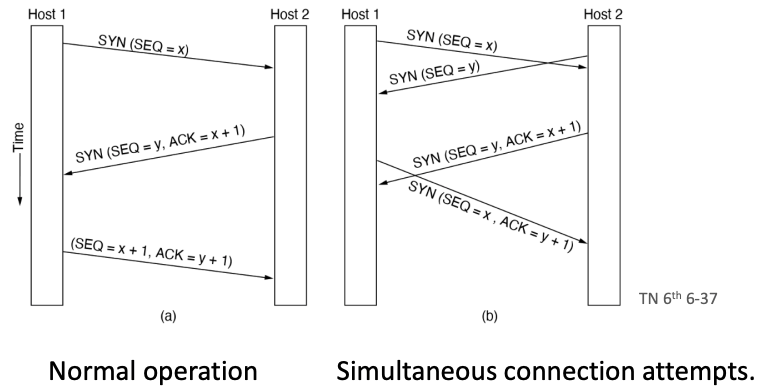
\includegraphics[width=\linewidth]{figs/three-way-handshake.png}

\subsection{TCP flow control}
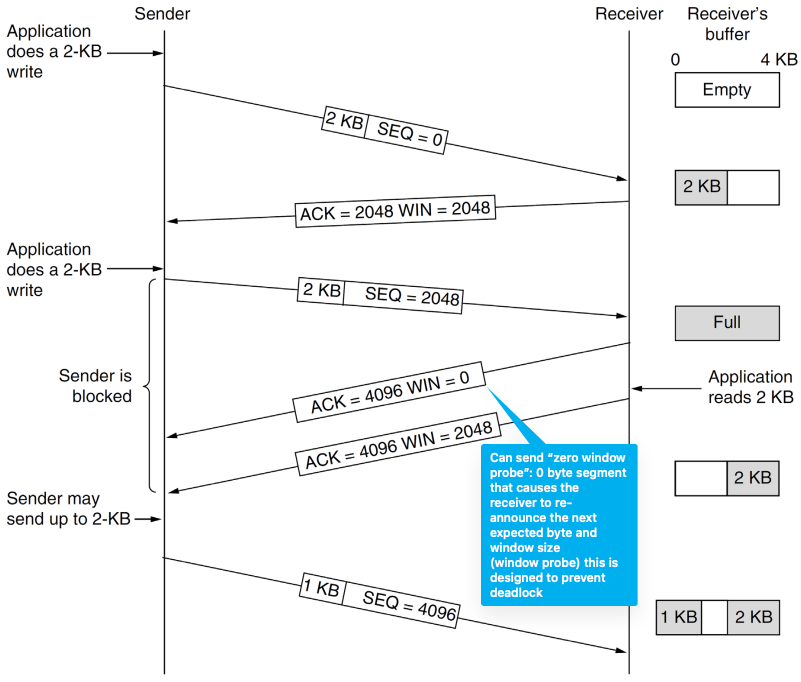
\includegraphics[width=\linewidth]{figs/tcp-sliding-window.png}
\textbf{Go-back-N:} when a packet is lost, retransmit all packets from the lost packet onwards. Receiver does not need to buffer out-of-order packets.\\
\textbf{Selective repeat:} (or fast retransmit) when a packet is lost, retransmit only the lost packet. Receiver needs to buffer out-of-order packets. Only helps if loss is common.\\

\subsection{TCP congestion control}
\textbf{Slow start:} increase congestion window size exponentially until a threshold.\\
\textbf{Round trip time:} time taken for a packet to be sent and acknowledged/received.\\

\subsubsection{Macroscopic model}
Let $W$ be the congestion window size, $p$ be the packet loss rate.\\
\textbf{Average increase in congestion window size:} $$\frac{(1-p)}{W} - p \frac{W}{2}$$
\textbf{Equilibrium point:} occurs when the average increase in congestion window size is zero.
$$\frac{(1-p)}{W} - p \frac{W}{2} = 0 \implies W \approx \sqrt{\frac{2}{p}}$$
\textbf{Rate:} $$\frac{W}{T} \approx \frac{1}{T} \sqrt{\frac{2}{p}} \text{ where } T = \text{round trip time}$$
This means for a given packet loss rate, the rate of increase of congestion window size is inversely proportional to the round trip time.\\

\subsection{Other layers}
\textbf{Presentation layer:} syntax and semantics of information exchanged between hosts.\\
\textbf{Session layer:} synchronization, checkpointing, recovery of data exchange.\\
\textbf{Transport layer:} reliable data transfer, congestion control, flow control.\\
\textbf{Transport layer encapsulation:} abstract representation of messages sent to and from transport entities.\\
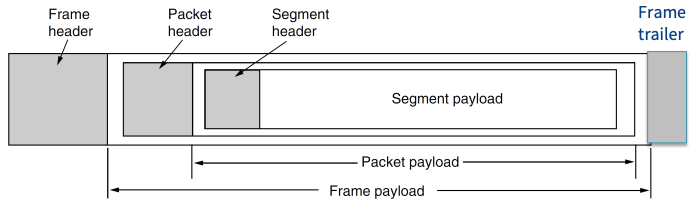
\includegraphics[width=\linewidth]{figs/encapsulation-of-segments.png}\\


\subsection{Packet switching, circuit switching}
\textbf{Packet switching:} a mode of data transmission in which a message is broken into a number of parts which are sent independently, over whatever route is optimum for each packet, and reassembled at the destination. The internet is a packet switched network.\\
\textbf{Packet forwarding (connectionless):} uses packet switching and must have a minimum required service of "send packet". This type of connectionless packet forwarding is called datagram network.\\
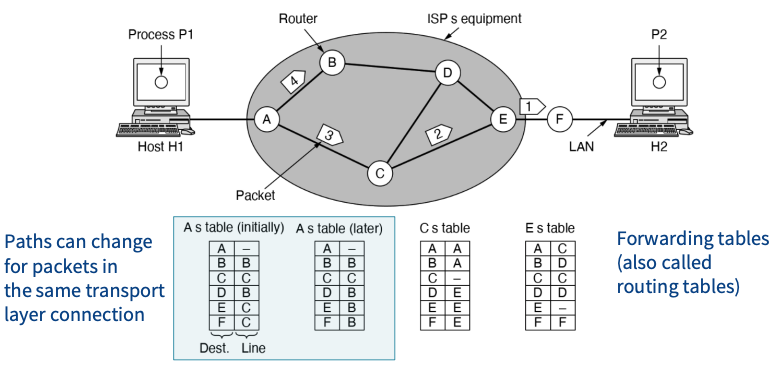
\includegraphics[width=\linewidth]{figs/packet-forwarding-connectionless.png}\\
\textbf{Packet forwarding (connection-oriented):} uses circuit switching and called virtual circuit network.\\
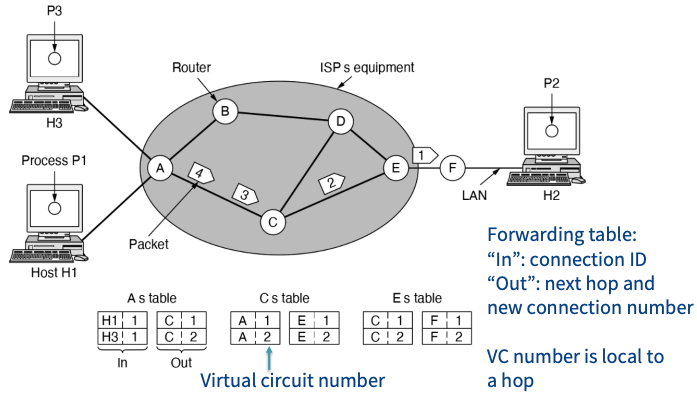
\includegraphics[width=\linewidth]{figs/packet-forwarding-connection-oriented.png}\\
